\textit{Определение} \textbf{N-граммы} представляют собой последовательности из \( n \) элементов в тексте или последовательности символов, где \( n \) обозначает количество элементов в последовательности. Элементы могут быть символами, словами или более крупными фрагментами текста в зависимости от контекста применения. Анализ n-грамм является важным методом в обработке естественного языка (Natural Language Processing, NLP) для изучения частотности последовательностей слов или символов в текстовых данных.

Формально, n-грамма \( \text{ngram}_n \) длины \( n \) в тексте \( T \) определяется как последовательность \( n \) элементов, где каждый элемент \( x_i \) может быть символом, словом или другими единицами текста:

\[ \text{ngram}_n = (x_1, x_2, ..., x_n) \]

Использование n-грамм в анализе текста позволяет оценивать частотность последовательностей слов или символов и изучать лингвистические характеристики текста, такие как структура, стиль и тематика. Кроме того, n-граммы могут использоваться в задачах моделирования языка, предсказания следующего слова в предложении, а также в машинном переводе и других приложениях обработки естественного языка.

\textit{Определение} \textbf{Токенизация} процесс в котором текст разбивается на токены. 
Это позволяет применить лемматизацию к каждому слову в тексте независимо от контекста.

Токенизация позволяет характерный порядок слова

 Лемматизация часто используется в различных областях NLP, включая информационный поиск, анализ тональности, машинный перевод и другие.

\textit{Определение } \textbf{Векторное вложение}(\textit{англ} embedding) векторное представление $\mathbb{R}^N$ слова $w$,
проявляеющие семантические и синтаксические при операциях сложения и взятия косинусного расстояния.

\begin{figure}[h]
    \centering
    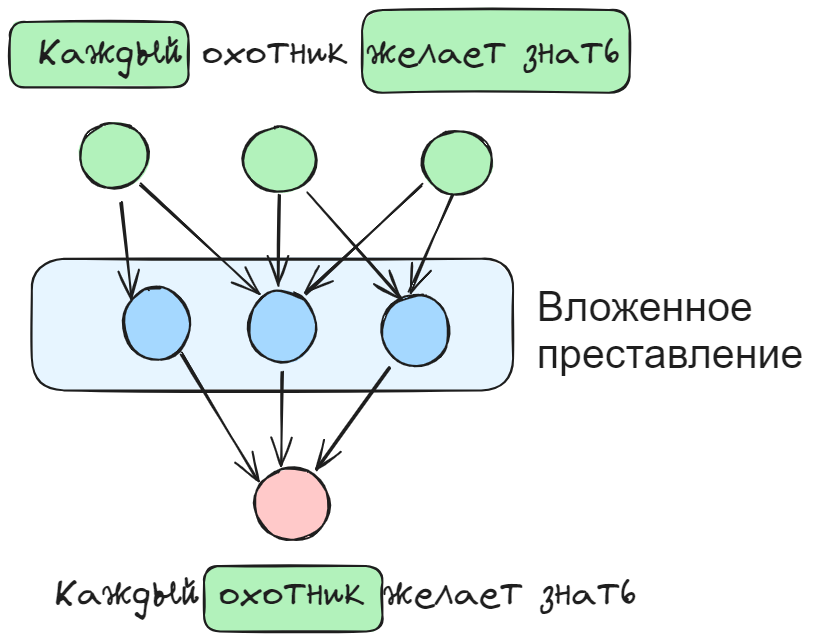
\includegraphics[width=0.5\textwidth]{assets/ml/nlp/word2vec.excalidraw.png}
    \caption{Векторное позволяет выполнять семантические операции}
    \label{embedding}
\end{figure}

Практически востребованной оказалась дистрибутивная гипотеза \cite{Schutze},
легшая в основу алгоритма Word2Vec (Вектор для Слова)\cite{NIPS2013_9aa42b31}. 
Известны и другие подходы GloVe, FastText, улучшающие подход
\begin{equation}
    \cos(\theta) = \frac{w_1 \cdot w_2}{\|w_1\| \|w_2\|}
\end{equation}
Векторные вложения слов играют важную роль в генеративном моделировании естественного языка, так как они позволяют моделям представлять слова в виде непрерывных числовых значений, которые могут быть использованы как входные данные для алгоритмов машинного обучения. 
Это позволяет моделям эффективно изучать зависимости между словами и генерировать тексты семантически богатые и лингвистически осмысленные.
\begin{figure}[h]
    \centering
    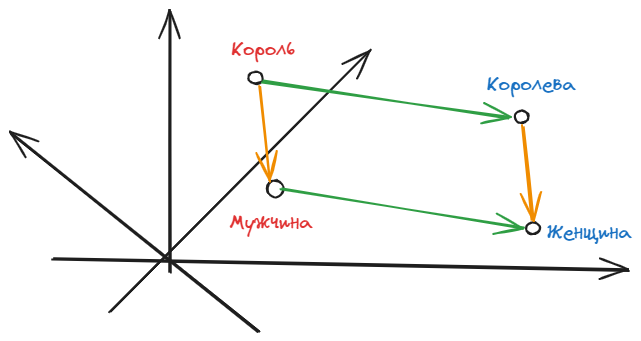
\includegraphics[width=0.5\textwidth]{assets/ml/nlp/vector.excalidraw.png}
    \caption{Векторное позволяет выполнять семантические операции}
    \label{embedding}
\end{figure}
Появление трансформерной архитектуры нейросетей  позволило улучшить результаты семантического представления до
работы с предложениями и параграфов \cite{devlin2018bert}.
\begin{figure}[h]
    \centering
    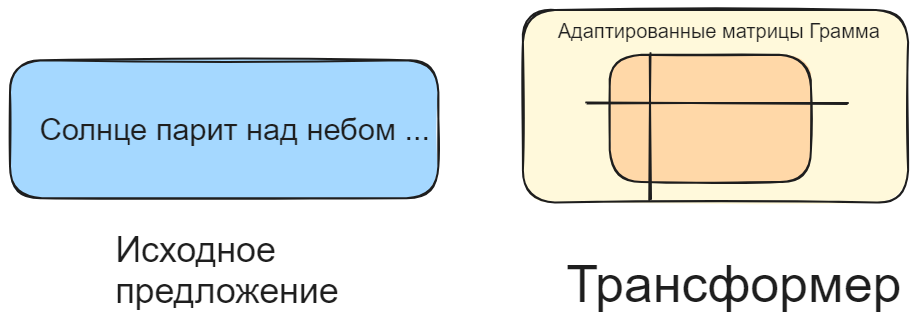
\includegraphics[width=0.5\textwidth]{assets/ml/nlp/bert.excalidraw.png}
    \caption{Векторное позволяет выполнять семантические операции}
    \label{embedding}
\end{figure}
Ключевым преимуществом модели является работа с максированным представлением языка, что позволяет изменить постановку обучения 
до предсказания промежуточного элемента.
\begin{equation}
    P(w_i |w_1,\dots,w_{i-1},w_{i+1},\dots, w_n) 
\end{equation}
Зада




